\chapter{Capitolo 1: Concetti base di biologia}
La bioinformatica è una materia che tratta tanto l'informatica quanto la biologia, pertanto è necessario illustrarne gli argomenti più importanti, che verranno spiegati in modo funzionale allo scopo della presente tesi.
\newline
La \textit{biologia} è la scienza che studia la vita, dagli attori che ne fanno parte fino ai processi in cui essi sono coinvolti. Poiché la vita nella terra si estende dalla biosfera fino alle molecole, si è resa necessaria l'esigenza di trovare una vera e propria scala a livello globale. Tra le varie forme di vita si trovano, omettendo quelle non interessate ed in ordine crescente, le molecole (insiemi di atomi), le macromolecole (insieme di molecole) e le cellule (insieme di macromolecole).
\newline
Ci sono quattro tipi di macromolecole che risultano essenziali per tutte le forme di vita:
\begin{itemize}
	\item \textit{Polisaccaridi}: macromolecole formate da un'insieme molecole, ovvero i monosaccaridi, tra cui il fruttosio, il glucosio e così via.
	\item \textit{Proteine}: sono la "struttura" degli esseri viventi, infatti consentono lo sviluppo e mantenimento degli organi.
	\item \textit{Lipidi}: chiamati anche grassi, sono le riserve di energia.
	\item \textit{Acidi nucleici}: DNA e RNA.
\end{itemize}
Di seguito vengono approfonditi il DNA e l'RNA.
\newpage

\section{DNA}
Il \textit{DNA} o \textit{acido desossiribonucleico} è una macromolecola contenente il patrimonio genetico degli esseri viventi. Il patrimonio genetico contiene tutte le informazioni genetiche\footnote{successivamente verrà mostrata la definizione di gene.} di un organismo.
\newline
Di seguito viene illustrata un'immagine del DNA, insieme ad una breve introduzione.
\newline
\begin{figure}[h!]
	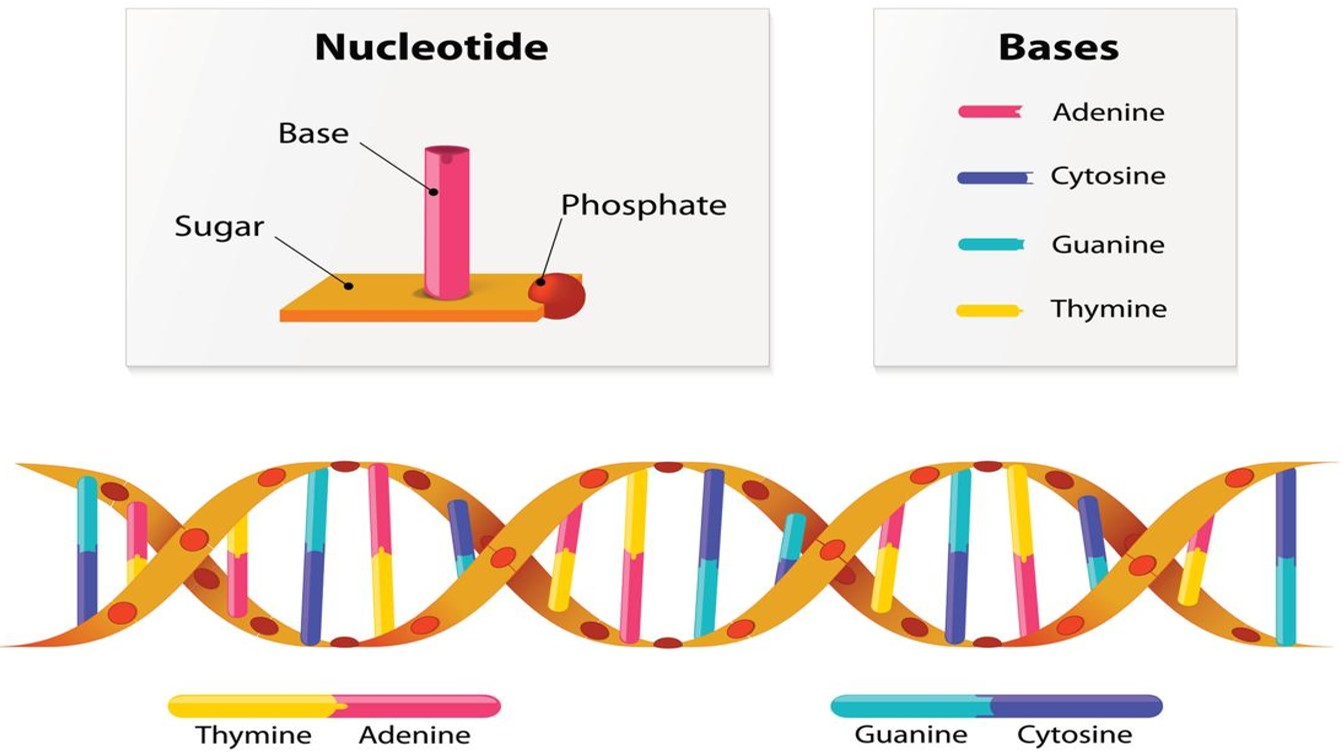
\includegraphics[width=\linewidth]{DNAStructure.jpg}
 	\caption{La struttura del DNA e del nucleotide.}
  	\label{fig:DnaAndNucleotideStructure}
\end{figure}
\newline
La struttura del DNA è ottimizzata per contenere informazioni, caratterizzata da una doppia elica dove ciascun filamento è formato da una \textit{sequenza di nucleotidi} dalla lunghezza variabile, che possono essere considerati i suoi "mattoncini".
\newline
Ciascun nucleotide è composto da una molecola di zucchero, un gruppo fosfato\footnote{Il gruppo fosfato è un un insieme di elementi strutturati e ben definiti} ed una base azotata. Queste ultime legano assieme i due filamenti del DNA, e è possibile trovarne di quattro tipi:
\begin{itemize}
	\item \textit{Adenina} (A)
	\item \textit{Timina} (T)
	\item \textit{Guanina} (G)
	\item \textit{Citosina} (C)
\end{itemize}
La base azotata Adenina si può legare solo la Timina (A-T), mentre la Guanina solo con la Citosina (G-C), questo significa che i filamenti sono complementari, e quindi se conosciamo le basi di un filamento sappiamo pure quelle dell'altro filamento(se una base azotata di un filamento è la Timina, allora la corrispondente base azotata dell'altro filamento è l'adenina).
TODO: descrivere brevemente il gene.

\section{RNA}
L'\textit{RNA}, è una macromolecola che sta per acido ribonucleico, caratterizzato da una struttura a singolo filamento composto da una \textit{sequenza di ribonucleotidi} più o meno lunga.
\newline
I ribonucleotidi si differenziano dai nucleotidi per una differente molecola di zucchero e perché la Timina (T) è sostituita con l'Uracile(U).
